\documentclass[journal]{IEEEtran}
%\IEEEoverridecommandlockouts
% The preceding line is only needed to identify funding in the first footnote. If that is unneeded, please comment it out.

% listings package for code blocks
\usepackage{listings}
\usepackage{xcolor}
\usepackage{cite}
\usepackage{verbatim}
\usepackage{graphicx}
\usepackage{parskip}

\begin{document}

% overfull \hbox .. too wide 
\setlength{\emergencystretch}{12pt}
%\setlength{\parskip}{0pt} % 1ex plus 0.5ex minus 0.2ex}
\setlength{\parindent}{10pt}

\definecolor{codegreen}{rgb}{0,0.6,0}
\definecolor{codegray}{rgb}{0.5,0.5,0.5}
\definecolor{codepurple}{rgb}{0.58,0,0.82}
\definecolor{backcolour}{rgb}{0.95,0.95,0.92}

\lstdefinestyle{mystyle}{
    backgroundcolor=\color{backcolour},   
    commentstyle=\color{codegreen},
    keywordstyle=\color{magenta},
    numberstyle=\tiny\color{codegray},
    stringstyle=\color{codepurple},
    basicstyle=\ttfamily,
    breakatwhitespace=false,         
    breaklines=true,      
    postbreak=\mbox{\textcolor{red}{$\hookrightarrow$}\space},           
    captionpos=b,
}

\lstset{style=mystyle}

\title{Comparing Classifications Models Against the Naïve Bayes Classifier and Linear Discriminant Analysis Model}

\author{
\IEEEauthorblockN{Lillian Mueller}
\IEEEauthorblockA{lmuelle1@umd.edu}
}

\maketitle

\begin{abstract}
\label{log:abstract}

Ranking the performance of a classification model can be difficult when there is not a benchmark to compare the performance to. Using the Iris dataset from Scikit-Learn, the Naïve Bayes Classifier was used as a benchmark to evaluate the performance of the decision tree model, logistic regression model, k-nearest neighbor model, and finally the linear discriminant analysis model. All models were found to be effective classifiers of the iris dataset and were confirmed through receiver operating characteristics and cross-validation. Overall, the linear discriminant analysis model proved to be most effective in classifying iris data. Through this investigation, the importance of using multiple model evaluation methods and determining a model performance benchmark was demonstrated. 

\end{abstract}

\section{Introduction}
\label{sec:intro}

Many classification models have been used and tested on the Iris dataset from Python's Scikit-Learn library. However, these models have only been compared to each other. Having a base line to compare a model to allows an analyst to determine whether a model performs well in general. In this investigation, the Naïve Bayes classifier was used as that baseline to test the prediction performance of the decision tree classification model, the logistic regression model, and the K-nearest neighbor (KNN) model. Additionally, a Linear Discriminant Analysis (LDA) was developed  to provide another classification model to compare the models against. All models are predicting the classification of each iris flower from the Iris dataset. This dataset consists of 3 classifications: setosa, virginica, and versicolor. The flowers' features used to discern its class include sepal width and length, and petal width and length. Using the benchmark, the analyst can determine which models are good predictors for the iris dataset as well as find the best model for the dataset. 

The naïve bayes classifier is similar to logistic regression models as it estimates the probability that a record belongs to one classification over another and bins it into the classification with the greatest probability \cite{b1}. However, the reason the naïve bayes classifier may serve as a benchmark is because it does not consider any interaction between the features; it assumes conditional independence. Additionally, this model is very efficient in computation time and storage which makes it an easy and inexpensive way to evaluate another model. 

Linear Discriminant Analysis (LDA) is most like decision tree where the algorithm finds linear combinations that best separates the classes in the dataset. However, where decision trees split the data into two groups at each node, effectively drawing a straight line the feature space, LDA find the direction that can best separate the classes \cite{b2}. This model may be a good fit for the iris data set as it has been shown the decision tree model is effective at predicting the classification of iris data.

The methodology followed to develop the Naïve Bayes classifier, LDA classifier and model comparisons are described in Section \ref{sec:methodology}. Results are discussed in Section \ref{sec:results}. And finally lasting comments and future research can be found in Section \ref{sec:discussion}.

\section{Methodology}
\label{sec:methodology}

This investigation entails using various classes from the library \lstinline{sklearn}. To develop the models: \lstinline{GaussianNB} class from the \lstinline{naive_bayes} module, the \lstinline{DecisionTreeClassifier} class from the \lstinline{tree} module, the \lstinline{LogisticRegression} class from the \lstinline{linear_model} module, the \lstinline{KNeighbors} function from the \lstinline{neighbors} module, and \lstinline{LinearDiscriminantAnalysis} class from the \lstinline{discriminant_analysis} module. Each was used to develop the naïve bayes classifier, decision tree model, the logistic regression model, KNN model, and the LDA respectively. To develop the ROC (receiver operating charactoristics) of each model,  \lstinline{sklearn}'s \lstinline{metrics} module was used. Other Python libraries used along the way to help handle the data include \lstinline{matplotlib.pyplot}, \lstinline{pandas}, and \lstinline{numpy}. 

First, the Iris dataset was loaded from the \lstinline{sklearn} library through the \lstinline{datasets.load_iris} function. A new column called “class” was added which contains the \lstinline{target} variable of the Iris dataset; this is the class of the Iris plant: setosa, versicolor, or virginica. Since the \lstinline{target} attribute contains an array with values from 0-2, the \lstinline{replace()} function was used to map these numerical values to their corresponding classifications: setosa for \(0\), versicolor for \(1\), and virginica for \(2\). 

After the Iris dataset was loaded in and processed, it was split into a train group and test group using the \lstinline{model_selection.test_train_split()} function, with 2/3 of the data as the train group and the remainder as the test group. 

Next, the models were developed. For the decision tree, logistic regression, and KNN models, similar methods were used as described in previous studies \cite{b3}-\cite{b5}. Regarding specific parameters, the decision tree model was developed with the Gini impurity criterion, the logistic regression model was developed without any penalty, and the KNN model was developed using k=10 and the Euclidean distance metric. These were determined to be the most effective version of each model in their respective investigation. Additionally, all models were trained using the same training subset of the dataset. For the naïve bayes classifier, the \lstinline{naive_bayes.GaussianNB()} class was used and trained on the same training dataset. For the linear discriminant analysis, the \lstinline{linear_discriminant.LinearDiscriminantAnalysis()} class was used and also trained on the training dataset. For each of these models, the classification report was created using the \lstinline{metrics.classification_report()} function which displays the accuracy, precision, and recall scores of the model overall and with respect to each classification. 

To compare the models, a ROC curve was created for each model to find the models AUC (area under the curve). This value is a scalar value that allows the user to evaluate the models performance with respect to false positives versus true positives and provides an easy way for the analyst to rank the classifiers. The methodology to develop the curves for each model is similar to the methodology explained in a previous report \cite{b6}.  However, since the iris dataset consists of 3 classifications rather than 2, the data had to be reconfigured to binarize the target using one-hot-encoding. This process uses a “one versus all” computing strategy where a single classification is presented as one class, and all the other classes are presented as another. For this investigation, the class showing the lowest precision values across the models was the versicolor class; this class was used to evaluate the ROC curves. Using the \lstinline{preprocessing.LabelBinarizer()} class, object was fit to the dataset. The object was then able to transform the targets (the true classifications) and predictions (classifications predicted by the model) into the binary classifications where the desired class was represented as 1, and all other classes were represented as 0. Using these transformed arrays, the false positive rate, the true positive rate, and the area under the curve values were calculated for each model using the \lstinline{metrics.roc_curve()} and \lstinline{metrics.auc()} functions. The false positive and true positives rates from each models were graphed using \lstinline{matplotlib.pyplot} and the AUC values were compared. 

Finally, to further validate and compare these models, each model was evaluated using cross-validation. Using 10 folds and the methodology found in a previous investigation, the mean accuracy and the standard deviation of all the accuracies from each fold were found and compared \cite{b7}.

\section{Results}
\label{sec:results}

Upon testing each model, the accuracy and precision of each model is as displayed in Table \ref{table:stats}. 

\begin{table}[h!]
\centering
\begin{tabular}{ c | c c c | c}
    Model & & Precision & & Accuracy \\ 
        & 0 & 1 & 2 \\
\hline
Naive Bayes & 1.0    & 0.79 & 0.86 & 88\% \\
Linear Discriminant Analysis  &    1.0    &    0.94   &  1.0 & 98\%\\
Decision Tree   &    1.0    &    0.80   &  0.92 & 90\% \\
Logistic Regression   &    1.0    &    0.86   &  0.74 & 86\%\\
K-Nearest Neighbor  &     1.0   &     0.94  &   0.94 & 96\%\\

\end{tabular}
\caption{Model Accuracy and Precision for Each Classification}
\label{table:stats}
\end{table}

Looking at these statistics alone, one may conclude that the LDA model is the best as it had the highest precision across the board and highest accuracy of 98\%. Additionally, from these results, the naïve bayes outperforms the logistic regression model. Of the three models, the decision tree, logistic regression, and k-nearest neighbor models, the k-nearest neighbor model preformed the best with an accuracy of 96\%. To get a better picture of the performance of each model, the ROC curves were developed. Figure \ref{fig:versicolor} shows the curves of each model on a single graph along with its AUC (area under the curve). 

\begin{figure}[h!]
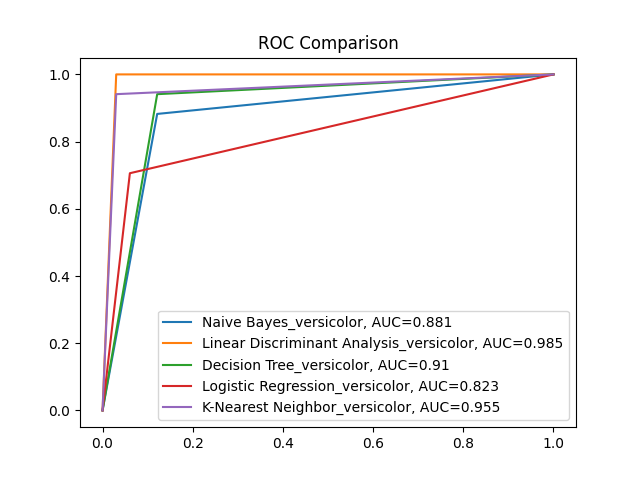
\includegraphics[scale=0.6]{rocCurves_versicolor.png}
\centering
\caption{ROC Curves for Versicolor Classification}
\label{fig:versicolor}
\end{figure}

Here, again the analyst can conclude the same rankings as before. A perfect model would have an AUC of 1. Each model displayed has an AUC of .8 or higher which means each model has some merit and is efficient at being a predictor of the iris dataset. The best model, with an AUC of .985 is the LDA model, followed by the KNN model with an AUC of .955. The third, fourth, and fifth best model were the decision tree model (AUC=.91), naïve bayes classifier (AUC=.881), and finally the logistic regression model (AUC=.823) respectively. If an analyst were using the Naïve Bayes model as a benchmark, the logistic regression model does not make the cut, whereas the decision tree and k-nearest neighbor are better than the benchmark in this case. 

\vspace{40px}

As the previous evaluation methods could have bias due to the training data and testing data split, cross validation was run on each model to determine a more holistic calculation of the accuracy. Table \ref{table:crossval}. 

\begin{table}[h!]
    \centering
    \begin{tabular}{c | c c}
        Model & Mean Accuracy & Standard Deviation \\
        \hline
        Naive Bayes	& 0.953	& 0.045 \\
        Linear Discriminant Analysis	& 0.980	& 0.045 \\
        Decision Tree	& 0.960	& 0.047 \\
        Logistic Regression	& 0.980	& 0.045 \\
        K-Nearest Neighbor	& 0.967	& 0.047 \\

    \end{tabular}
    \caption{10-Fold Cross Validation Results}
    \label{table:crossval}
\end{table}

These results tell a very different story. The LDA and logistic regression model prove to be the most accurate. The naïve bayes classifier is the least accurate. When using the Naïve bayes as a benchmark for a well performing model, all models prove to be better than the base case. The rankings from the cross-validation results are as follows: 
\begin{enumerate}
    \item LDA and Logistic Regression
    \item KNN
    \item Decision Tree 
    \item Naïve Bayes
\end{enumerate}

These rankings are more reliable than previous as the cross-validation method is not as influenced by the balance of the training and testing datasets. From both these methods however, the LDA model proves to be the best model for the iris dataset. 

\section{Discussion}
\label{sec:discussion}

Overall, it was expected that the models would be proven effective. The naïve bayes classifier used as the benchmark in this investigation was deemed less than the decision tree, KNN, LDA, and logistic regression models. The analyst can conclude that the LDA model was the best fit for this dataset as it was the best performing model in all evaluation methods. However, what was unexpected was the vast difference between the evaluation methods. When using the AUC of the ROC curves as a metric to rank the classifiers, it seemed the logistic regression model was the worst of the models as its AUC was less than that of the naïve bayes classifier model. After evaluating the models via cross-validation, it became clear that the logistic regression model was far from being less effective than the naïve bayes classifier. The logistic regression model was the most accurate of the models. This demonstrates how important it is to evaluate the performance of any model through more than one method. By only using the ROC curve analysis and not include the LDA model, the overall better performing logistic regression model would have been overlooked and the KNN model may have been deemed the best model for the dataset. 

In both evaluation cases however, there was a model that rose to the top: the LDA. This investigation demonstrates the LDA model is the best fit for the data. It had the greatest AUC value and the greatest average accuracy. In the future, it is worth investigating why the cross-validation accuracy of the LDA and the logistic regression model were equal when the AUC values of each model were so different. It is clear that the AUC evaluation relies greatly on the training and testing dataset. Examining how to reduce this bias would greatly benefit future comparisons using this method so the analyst has a better scope of the model's performance when it comes to dealing with true positives versus false positives. 

\begin{thebibliography}{00}
\bibitem{b1}{F. Provost and T. Fawcett, Data Science for Business: What You Need to Know About Data Mining and Data Analytic Thinking, First edition (2005). }
\bibitem{b2}{“ML | Linear Discriminant Analysis,” GeeksforGeeks. Accessed: Nov. 17, 2023. [Online]. Available: https://www.geeksforgeeks.org/ml-linear-discriminant-analysis/}
\bibitem{b3}{L. Mueller and R. Hong, “Investigating Decision Trees”.}
\bibitem{b4}{L. Mueller and R. Hong, “Iris Classification Using Logistic Regression”.}
\bibitem{b5}{L. Mueller and R. Hong, “Evaluating the Performance of K-Nearest Neighbors Classification”.}
\bibitem{b6}{L. Mueller, “Ranking Classification Models using Receiver Operating Characteristics”.}
\bibitem{b7}{L. Mueller and R. Hong, “Using K-Fold Cross Validation on Decision Tree and Logistic Regression Models to Classify Iris Species”.}

\end{thebibliography}

\end{document}